\documentclass{article}[11pt]
\usepackage{graphicx}
\usepackage{tabularx}
\usepackage{natbib}


\usepackage{array}
\usepackage{amsmath}
%\usepackage[backend=bibtex]{biblatex}
\bibliographystyle{..//refs/styles/besjournals.bst}
\setkeys{Gin}{width=0.8\textwidth}
%\setlength{\captionmargin}{30pt}
\setlength{\abovecaptionskip}{10pt}
\setlength{\belowcaptionskip}{10pt}
 \topmargin -1.5cm 
 \oddsidemargin -0.04cm 
 \evensidemargin -0.04cm 
 \textwidth 16.59cm
 \textheight 21.94cm 
 \parskip 7.2pt 
\renewcommand{\baselinestretch}{1.5}
\AtBeginEnvironment{thebibliography}{\linespread{1}\selectfont}
\parindent 0pt
\usepackage{lineo}
\linenumbers % for dissertation
\pagenumbering{gobble}% for dissertation
%\usepackage{xr}
\usepackage{xr-hyper}
\usepackage{hyperref}
\externaldocument{SUPPinvasive}

\title{Phenological responses to climate mediate seedling competition with
an invasive woodland herb}
%EMWAug2022: Tossing out a new idea at the last miniute

\author{D.M. Buonaiuto $^{1,2,3a}$, E.M. Wolkovich$^{2,3,4}$}
\date{}
\usepackage{Sweave}
\begin{document}
\input{invasive-concordance}
\maketitle
\noindent \emph{Author affiliations:}\\
\noindent $^1$Department of Environmental Conservation, University of Massachusetts, Amherst, Massachusetts, USA. ORCID: 0000-0003-4022-2591\\
\noindent $^2$Arnold Arboretum of Harvard University, Boston, Massachusetts, USA.\\
$^3$Department of Organismic and Evolutionary Biology, Harvard University, Cambridge, Massachusetts, USA \\
$^4$Forest \& Conservation Sciences, Faculty of Forestry, University of British Columbia, Vancouver, British Columbia, Canada\\
$^a$Corresponding author: 617.823.0687; dbuonaiuto@umass.edu\\

\pagebreak
\section*{Abstract}
\begin{enumerate}
\item Invasive plants are often characterized by rapid germination and precocious phenology. Theory suggests that early germination may provide invaders with competitive advantage over slower germinating natives, but the relative contribution of rapid germination vs. other intrinsic competitive traits to the success of invaders is poorly understood. Depending on the relationship between germination and competition, shifts in germination phenology due to climate change may increase the dominance of invaders or buffer communities against their impacts. %Predicting invasion dynamics and the structure and function of plant communities of the future requires clarifying the relationship between climate variability, phenology and competitive outcomes.

\item We investigated the link between temperature variation, germination phenology and competitive interactions with a sequence of controlled environment experiments. First, we evaluated the relationships between temperature variation and germination phenology for two North American herbaceous species, the invasive \textit{Hesperis matronalis} and native \textit{Cryptotaenia canadensis}. We then leveraged temperature-response differences to manipulate the relative germination phenology of these taxa and quantified the effects of their phenological differences on competition.

\item Seeds of the invasive \textit{H. matronalis} germinated rapidly, reaching 50\% germination in under ten days in all treatment combinations.\textit{C. candensis} did not reach 50\% germination with less than seven weeks of cold stratification. However, with more than 10 weeks of cold stratification and low (20/10$^{\circ}$C) incubation temperatures, the germination phenology of \textit{C. canadensis} was well matched to that of \textit{H. matronalis}. When grown together, we found that precocious germination phenology doubled the competitive impact of \textit{H. matronalis} relative to its other intrinsic competitive traits. Phenological advantage of just two-three days relative to \textit{C. canadensis} was enough to secure competitive dominance at the seedling stage. %The germination phenology of most native species in our study was strongly associated with cold stratification. 
%The strong temperature dependence of the competition dynamics we observed suggest that global warming will likely increase the phenological advantage of rapidly germinating invaders due to the stronger effects of temperature variation on the phenology of native plants compared with their invasive competitors.
%work on below
\item \textit{Synthesis and applications.} This study revealed that the mechanistic link between the germination phenology and competitive success of an invasive plant can be strongly mediated by climate sensitivity differences between introduced and native species. Climate change will likely exacerbate these differences, especially in regions where warming reduces the cold stratification. Our findings suggest that phenological diversity in native plant communities is an important property of invasion resistance. The relationship between environmental variation, germination dynamics and competition provide a path forward for forecasting climate change impacts on seasonal community assembly, and highlights the need to incorporate phenological diversity in restoration.

\end{enumerate}
%350 words

Keywords: competition, climate change, germination, invasion, phenology, priority effects, stratification

\pagebreak
\section*{Introduction}
 A central tenet of community assembly theory is that the order of arrival of species mediates inter-specific interactions and can dictate the trajectory of community structure \citep{Fukami2015}. These historical contingencies, known as priority effects, alter the structure and function of communities, driving communities to long-term alternate stable states \citep{Fukami2011}. Yet in many ecosystems, plant communities must re-assemble each year after a period of dormancy. In these communities, priority effects are the products of phenology, the timing of seasonal life cycle events, % and the rate at which dormant plants and seeds respond to their environment and resume growth or germinate when favorable conditions return 
rather than the timing of the arrival of propagules, which occurs prior to the dormant season in many cases \citep{Rudolf:2019aa,Howe:1982aa,Baskin:1988aa}. 
%These seasonal, or short-term priority effects \citep{Wainwright_2011,Young:2017aa}, may be important mediators of plant interactions, and have been invoked to explain the competitive dominance of some species (when strong competitors also have rapid/early germination) \citep{Gioria2018}, and inter-specific coexistence (when weaker competitors have rapid/early germination and/or priority varies over time) \citep{Towers:2020aa}.

Invasive plants are often characterized by rapid germination and precocious phenology under a wide variety of environmental conditions \citep{Gioria2018,Gioria:2017wo,Wolkovich:2011uh,Smith:2013uj}. By contrast, native plants tend to exhibit more constrained germination cues \citep{Marushia:2010ug,Wainwright:2013tv,Van-Clef:2001to}. In many temperate systems, seeds of native plants are dispersed with deep physiological dormancy, requiring prolonged exposure to specific environmental conditions, such as cold stratification (cool temperatures of 0-10$^{\circ}$ C), to break dormancy and stimulate germination \citep{Brink:2013wr,Cavieres:2017aa,Bradford:2007tj}.

These differences in germination physiology can yield strong differences in the relative germination phenology of invasive and native plants, with invaders germinating well before their native competitors \citep{Gioria:2017wo}. This difference in relative germination timing among species, which we refer to as \textbf{phenological advantage}, can contribute significantly to the competitive abilities, and ultimately invasion success, of invasive plants. By allowing them to begin drawing down seasonal resources and modifying their environment before their native competitors emerge \citep{Kardol2013}, invaders gain a competitive advantage through a \textbf{seasonal priority effect} \citep{Wainwright_2011}.

Despite the growing interest in seasonal priority effects, it has been difficult to quantify their overall contribution to the competitive success of invaders. Germination is notoriously difficult to monitor in the field, and rapid phenology often co-varies with other competitive traits \citep{Dickson2012,Milbau:2003vt,HAO:2009vh}. % such as high fecundity, growth rates, and stress tolerance 
Because of these difficulties, many experiments vary phenological advantage by sowing competing seeds at different time intervals \citep{Young:2017aa}. While these experiments have provided strong evidence that phenological advantage---on the order of just days to weeks---can yield substantial priority effects \citep{Weidlich:2020aa}, their experimental set-up is difficult to translate into natural communities in which priority effects are mediated by climate, and difficult to use for forecasting. %As such, the relative importance of phenological advantage vs. other competitive traits to invasion success and competition dynamics in nature remains poorly characterized. 
Understanding the role that phenological advantage plays in mediating the dynamics of interspecific competition is critical for predicting and managing the structure and function of plant communities in the face of anthropogenic climate change. 

Due  to interspecific differences in responses to environmental variation, sustained alterations to environmental conditions are already shifting community-wide patterns of germination \citep{Walck2011}. If patterns of germination are indeed tightly linked to the competitive dynamics of communities, then phenological re-organization is likely to shift the strength of species' interactions, change patterns of invasion, and strongly influence biological filtering of plant communities. 

In this study, we generated contrasting levels of phenological advantage among two woodland herbaceous species (the North American invasive \textit{Hesperis matronalis} and native \textit{Cryptotaenia canadensis}) by leveraging their differences in germination timing in response to environmental variation. First, we performed a series of germination assays in controlled environments under varying temperature regimes to estimate a realistic range of climate-driven variation in phenological advantage. % for a suite of widespread invasive and native forbs. 
We then used competition trials under contrasting environmental conditions to indirectly manipulate the phenological advantage between these two taxa and quantify the contribution of seasonal priority effects to their competitive dynamics. By linking climate variation, phenological advantage, and seasonal priority effects, our study has important implications for how anthropogenic climate change will alter phenological assembly and, in turn, plant community interactions in the decades to come.

\section*{Materials and Methods}

\subsection*{Focal species}
 For this study, we focused on a pair of woodland herbaceous species. Dames Rocket (\textit{Hesperis matronalis}) is a herbaceous biennial/perennial species in the \textit{Brasicaeceae} family, originally from Eurasia, and introduced to North America in the 19th century \citep{Francis:2009wz}. It  can rapidly invade  meadows, forest edges and woodlands, forming thick stands and excluding native vegetation \citep{Francis:2009wz}. It is currently listed as a noxious or invasive weed is several states and provinces in the United States and Canada \citep{Susko:2008ut}. Honewort (\textit{Cryptotania canadensis}) is a herbaceous perennial in the \textit{Apiaceae} family, native to forests and woodlands of eastern North America \citep{Hawkins:2007vb}. The  habitat overlap of these two species suggests that they may compete in nature. While their habitat requirements may be similar, the two species display a substantially different germination niche, making them a suitable model for our study. \textit{C. canadensis} seeds are classified with deep physiological dormancy and require a substantial period of cold moist stratification to release dormancy and initiate germination \citep{Baskin:1988um}. While some reports suggests that cold stratification enhances germination in \textit{H. matronalis} at low incubation temperatures, several studies have demonstrated that fresh and after-ripened (dry-stored) seeds of \textit{H. matronalis} are capable of rapid and complete germination at a wide range of temperatures \citep{Susko:2008ut}. %These contrasting germination dynamics among species suggest that phenological advantage between them is likely to be strong mediated by cold stratification and incubation variation.  

\subsection*{Experiment I: Germination Assays}
To investigate the relationship between environmental variation and relative germination timing among species, we obtained seeds of \textit{C. canadensis} from Prairie Moon Nursery (Winona, MN) and seeds of \textit{H. matronalis} from American Meadows (Shelburne, VT). %of 14 spring-germinating herbaceous species common to temperate forest-edges from domestic plant nurseries (see Tab. \ref{tab:specs} for details). 
We performed germination assays in the growth facilities of the Arnold Arboretum in Boston, Massachusetts, USA (42.3074$^{\circ}$ N, 71.1208$^{\circ}$ W). We assigned seeds to a fully-crossed set of twenty experimental treatments; 10 levels of of cold stratification duration (0,2,4,5,6,7,8,9,11,13 weeks at 4$^{\circ}$C) and two levels of incubation temperature (warm--- 25$^{\circ}$C:15$^{\circ}$C (day/night), cool--- 20$^{\circ}$C:10$^{\circ}$C (day/night)).

\noindent  Prior to applying experimental treatments we performed a ``float test" in which all seeds were placed in distilled water, and unfilled seeds (floating) were removed from the experiment \citep{Baskin2014}. We imbibed the remaining seeds in distilled water for 24 hours and then placed 20 seeds for each species/ treatment combination in petri dishes on moist pool-filter sand, with three replicates per treatment. For the cold stratification treatments, we wrapped petri dishes in aluminum foil to prevent light exposure and placed them in a growth chamber at 4$^{\circ}$C. After each stratification interval, we transferred the petri dishes to their assigned incubation chamber for 25 days, moistening the germination substrate as necessary to maintain maximum saturation of the medium without flooding the seeds. We checked for new germinates every two days, defining a seed as germinated when its radical or cotyledon tissue was visible \citep{Baskin2014}. We assessed the viability of any seeds that did not germinate in the 25 day incubation period by performing a ``crush test" in which we applied pressure to the intact seed to evaluate its condition \citep{Baskin2014}. We excluded any seeds deemed unviable from all subsequent analyses. Due to the staggering of our stratification treatments the experiment took place between 27 August - 12 December 2018.

\subsection*{Experiment II: Competition Trials}
\noindent To quantify the contribution of seasonal priority effects to interspecific competition dynamics we performed competition trials under controlled conditions in a research greenhouse at the Arnold Arboretum from October 2020 - February 2021. %For this experiment we selected two focal species from our germination assays, the North American invader Dames Rocket (\textit{Hesperis matronalis})  and native forb Honewort (\textit{Cryptotania canadensis})}. \textit{H. matronalis} is a herbaceous biennial/perennial species in the \textit{Brasicaeceae} family, originally from Eurasia, and introduced to North America in the 19th century \citep{Francis:2009wz}. It  can rapidly invade  meadows, forest edges and woodlands, forming thick stands and excluding native vegetation \citep{Francis:2009wz}. It is currently listed as a noxious or invasive weed is several states and provinces in the United States and Canada \citep{Susko:2008ut}. \textit{C. canadensis} is a herbaceous perennial in the \textit{Apiaceae} family, native to forests and woodlands of eastern North America \citep{Hawkins:2007vb}. These species share similar habitat, likely competing in nature. However, the two species display a substantially different germination niche, making them a suitable model for our study. \textit{C. canadensis} seeds are classified with deep physiological dormancy and require a substantial period of cold moist stratification to release dormancy and initiate germination \citep{Baskin:1988um}. While some reports suggest that cold stratification enhances germination in \textit{H. matronalis} at low incubation temperatures, several studies have demonstrated that fresh and after-ripened (dry-stored) seeds of \textit{H. matronalis} are capable of rapid and  complete germination at a wide range of temperatures \citep{Susko:2008ut}. These contrasting germination dynamics among species suggest that phenological advantage between them is likely to be strongly mediated by cold stratification and incubation variation.  
We planted seeds of \textit{C. canadensis} and \textit{H. matronalis} into 8.9 cm square pots, employing a response surface design where we varied both the overall density of seeds and proportion of each species in each pot \citep{Inouye2001}. High and low density treatments consisted of 14 and 8 seeds respectively. Proportion treatments were 100:0\%, 25:75\%, 50:50\%, 75:25\%, 0:100\% (\textit{C. canadensis}:\textit{H. matronalis}). Each density by proportion treatment was replicated six times. %This design allows us to evaluate effects of inter- and intra- specific competition and density dependence independently and in association with our experimental treatment.\\

\noindent We randomly assigned half of the pots to low (45 days) and high (72 days) cold stratification treatments in dark growth chambers at 4$^{\circ}$C. We staggered the start of the treatments, so that at the conclusion of the cold stratification, all pots were transferred to a heated greenhouse maintained at 15-25$^{\circ}$C with 14 hours of supplemental light. Germination was observed daily from 24 December 2020 - 13 January 2021 and every two days from 15 January 2021 - 01 February 2021. The locations of each pot in the greenhouse were randomly reassigned every three days to minimize any blocking effects on germination or growth.

\noident After 35 days we added 1 tsp per gallon of water of Peter’s 20-10-20 liquid feed fertilizer to all pots. After 62 days, we harvested the above-ground biomass from all pots, dried it for 48 hours at 60$^{\circ}$C, and recorded the dry weight of each species/pot.% using a Mettler balance.

\subsection*{Statistical analysis}
\subsubsection*{Germination Assays}
To assess interspecific differences in the relationship between germination rate and temperature variability, we fit a Bayesian mixed-effect accelerated failure time model \citep[AFT,][]{ONOFRI:2010tl} using a Weibull distribution for the likelihood function. We included weeks of stratification and incubation temperature and their interaction with species as fixed effects. The model written below is modified from \citet{ONOFRI:2010tl}.

$t_{50} &= t_0 \phi$

where $t_{50}$ is time to 50\% germination and corresponds to the germination times of a references seed lot ($t_0$) multiplied by and ``acceleration factor" ($\phi$). The acceleration factor is a product of the experimental treatments of our study through the equation:

$\phi=exp(\beta_{sp}X_{sp} &+\beta_{strat}X_{strat} &+ \beta_{inc}X_{inc} &+ \beta_{stratXspecies}X_{strat}*X_{sp} &+ \beta_{incXspecies}X_{inc}*X_{sp} )$

where $X_{sp}$, $X_{strat}$ and $X_{inc}$ are the species, stratification and incubation treatment levels in our experiment, and  $\beta_{sp}$, $\beta_{strat}$, $\beta_{inc}$, $\beta_{stratXspecies}$ and $\beta_{incXspecies}$ are the estimated effects on $\phi$  for adding an additional week or stratification or degree of incubation for each species respectively.  

The AFT modeling framework let us robustly compare germination timing (t50,  time to 50\% germination) even among treatments with different final germination percentages by accounting for viable seeds that did not germinate during our incubation window \citep{Soltani:2015aa,ONOFRI:2010tl}. One drawback of this approach is that this class of models assumes that all viable seeds will eventually germinate, which we would not expect in nature. For this reason, we considered any estimated t50 values greater than 40 days to indicate that seeds would not reach 50\% germination under those conditions.  

\subsubsection*{Competition trials}
\noindent We quantified phenological advantage between species by subtracting the mean germination time of \textit{H. matronalis} from that of \textit{C. canadensis} in each pot. This allowed us to evaluate the effect phenological advantage with a regression design \citep{Cottingham:2005ud}, with advantage values ranging from -1.3 to 9.5 (\textit{C. candensis} mean germination time 1.3 days earlier to 9.5 days later than \textit{H. matronalis}).

For each pot, we calculated the relative growth rate difference (RGRD) among species using the equation below, modified from \citet{Connolly2005}.\\

RGRD &= $ ln(\frac{Y_{Cc}}{y_{Cc}}) &- ln(\frac{Y_{Hm}}{y_{Hm}}) $\\

where $Y_{Hm}$ and $Y_{Cc}$ are the final biomass of the species at the end of the experiment and $y_{Hm}$ and $y_{Cc}$ are the initial biomass of the seeds planted at the outset of the experiment. For this calculation we obtained estimates of seed mass for our focal species from the Kew Gardens Seed Information Database \citep{kew}.  

We then modeled the effect of seedling density of \textit{C. canadensis}, \textit{H. matronalis} and phenological advantage using on RGRD. The model is written below:\\

$RGRD_i &= N(\alpha + \beta_{Hm}n_{Hm} + \beta_{Cc}n_{Cc} + \beta_{pri}MGT, \sigma_{RGRD}^2$)\\

where  $\beta_{Hm}$ and $\beta_{Cc}$ are known as the species influence parameters---representing the intrinsic competitive ability of each species---or the estimated effect of increasing the seedling density of each species by one individual on the RGRD \citep{Connolly2005},  and $\beta_{pri}$ is the priority effect, or the effect of increasing the difference in mean germination time between  \textit{H.matronalis} and \texti{C. canadensis} by one day. $n_{Hm}$ and $n_{Cc}$ are the number of germinated individuals of \textit{H. matronalis} and \textit{C. canadensis} respectively. In this formulation, $\alpha$ is an un-interpretable intercept \citep{Connolly2005}.

To assess whether the rapid germination phenology of \textit{H. matronalis} modified the germination niche of \textit{C. canadnesis} we performed two additional Bayesian regression analyses. We assessed the influence of planting type (single species vs. mixed competition) on the likelihood of \textit{C. canadensis} germination using a Bernoulli likelihood distribution and the mean germination time of \textit{C. canadensis} using a Gaussian likelihood distribution. In both models we included stratification treatment as a fixed-effect co-variate.

\subsection*{Model Implementation}
\noindent We fit all models using the R package ``brms" \citep{Burkner2018}.  We ran the model on four chains with 4000 iterations and a 3000 iteration warm-up for a total of 4000 posterior draws for each parameter, using weakly informative priors. We validated model performance by obtaining $\hat{R}$ values between 1 and 1.01, high effective sample sizes and no divergent transitions. For all models we report the mean posterior estimate along with 90\% uncertainty intervals (I_{90}).

\section*{Results}
\subsection*{Germination advantage}
%Across all species in our germination assays, the time to 50\% germination advanced by 6.14 days per week of cold stratification (converted from log scale; mean: -0.14, $CI_{90}:$\textit{-0.20, -0.08}), though the strength of this effect varied strongly among species  (Fig. \ref{fig:musurv}a, Fig. \ref{fig:AFTall}). The overall estimated effect of incubation temperature on germination phenology was weak, delaying time to 50\% germination by 1.45 days per $^{\circ}$C (converted from log scale; mean: 0.03, $CI_{90}:$\textit{-0.04, 0.10}), but this was due to strong inter-specific differences in the directional response to increasing incubation temperatures. The germination phenology of five species advanced with increasing incubation temperatures, and was delayed for six species (Fig. \ref{fig:musurv}b).%  suggesting that for these species, our warm incubation treatment exceeded their thermal optimum.\\
%Considering our focal species, 
\textit{H. matronalis} reached 50\% germination in under ten days for all environmental treatments, always exceeding 75\% germination regardless of environmental conditions (Fig. \ref{fig:aft}, Tab. \ref{tab:germcomps}). Increasing cold stratification duration and incubation temperature only marginally enhanced the germination rate of this species (Fig. \ref{fig:aft}). By contrast, increasing incubation temperature had a delaying effect on the germination rate of \textit{C. canadensis}, suggesting that the mean 20$^{\circ}$C temperature of our warm incubation treatment is supra-optimal for the species (Fig. \ref{fig:aft}). Without sufficient cold stratification ($<$7 weeks for low incubation and $<$10 weeks for high incubation temperatures), seeds of  \textit{C. canadensis} did not reach 50\% germination during the duration of our experiment (Fig. \ref{fig:aft}, Tab. \ref{tab:germcomps}). However, under high levels of cold stratification germination rates of \textit{C.canadensis} began to converge on those of \textit{H. matronialis}, and at levels of stratification $>$10 weeks and low incubation, the germination rate and fraction of \textit{C.canadensis} was well matched to that of \textit{H. matronalis} (Fig. \ref{fig:aft}, Tab. \ref{tab:germcomps}).
%
%Given the strong inter-specific differences in phenological sensitivity to stratification and incubation, our results indicate that climate strongly shapes patterns of phenological assembly, and patterns of phenological advantage can be highly variable due to climate variation.

\subsection*{Germination priority effects}
In the absence of phenological advantage, the influence  of adding one seedling of \textit{H. matronalis} to a pot community was almost 4X less than adding one \textit{C. canadensis} seedling on the pot-level RGRD (represented by the species' influence parameters---\textit{H. matronalis} ($\beta_{Hm}$): 0.13, $I_{90}$: \textit{0.08,0.17}, \textit{C. canadensis} ($\beta_{Cc}$): -0.40, $I_{90}$: \textit{-0.46, -0.35}). Each day increase in the phenological advantage of \textit{ H. matronalis} had approximately the same influence on shifting the community biomass composition towards \textit{H. matronalis} as adding an individual of that species to the community (seasonal priority effect ($\beta_{pri}$): 0.15, $I_{90}$: \textit{0.09, 0.20}, Fig. \ref{fig:RGRD}, Tab. \ref{tab:RGRD}). Together, these results suggest that \textit{H. matronalis} will come to dominate the community biomass composition unless \textit{C. canadensis} is at high relative abundance or the phenological advantage of \textit{H. matronalis} is small. %(Fig. \ref{fig:3D}).

\subsection*{Priority effects and germination niche modification}
We observed no evidence that the rapid germination of \textit{H. matronalis} adversely modified the germination niche of \textit{C. canadensis}. Neither the likelihood of germination nor the mean germination time of \textit{C. canadensis} were suppressed when the species grew in mixed-species competition vs. single-species pots (Fig. \ref{fig:nichemod}). Rather, at low stratification levels, the presence of rapidly germinating \textit{H. matronalis} might have positively affected the germination fraction of \textit{C. canadensis}, (\textit{C. canadensis} germination percentage is higher in competition pots under low stratification, Fig. \ref{fig:nichemod}a), though there is high uncertainty in this comparison.

\section*{Discussion}
%\subsection*{Germination advantage as a seasonal priority effect} 
\subsection*{Environmental drivers of seasonal priority effects}
Our experimental results advance the understanding of the role of seasonal priority effects on competition by identifying a natural mechanism, species' differential sensitivity to temperature, that can generate seasonal priority effects. In the absence of phenological advantage, the intrinsic competitive abilities of each species suggest that the native species, \textit{C. canadensis}, is the stronger competitor (Fig. \ref{fig:RGRD}). % $\beta_{2}$--- the influence parameter of \textit{C. canadensis} is significantly more negative than than $\beta_{1}$--- the influence parameter of \textit{H. matronalis}, is positive). 
However, the influence of one day of phenological advantage for \textit{H. matronalis} virtually doubled its influence on the final community composition, suggesting that seasonal priority effects play a major role in the competitive success of \textit{H. matronalis} (Fig. \ref{fig:RGRD}). Our results indicate that \textit{C. canadensis} can compete with the invasive \textit{H. matronalis} at high relative abundance levels and/or when phenological advantage is low, joining a growing body of experiments demonstrating that relative germination phenology can function as a seasonal priority effect, enhancing the performance of the earliest germinating species at the expense of later germinants \citep{Korner2008,Dickson2012,Ross1972}.

The role of seasonal priority effects in plant competition has been primarily demonstrated in experiments in which the planting of competing seeds is staggered at increasing intervals \citep{Young:2017aa,Weidlich:2020aa}. In our experiment, variation in phenological advantage was a product of interspecific differences in germination responses to cold stratification, suggesting that seasonal priority effects can strongly influence seedling competition even in environments were germination phenology is under strong temperature control. While it is possible that \textit{H. matronalis} interacts differently with other species, the results of our pair-wise competition trial suggests that seasonal priority effects, manifested through rapid germination phenology and propagule pressure, are mechanistically related to the competitive dominance, and---ultimately---invasion success of \textit{H. matronalis}. 

Our competition trials did not suggest any evidence that the rapid germination phenology of \textit{H. matronalis} impacted the germination niche of \textit{C. canadensis} (Fig. \ref{fig:nichemod}). This indicates that the mechanism underlying the seasonal priority effect of \textit{H. matronalis} is likely niche preemption \citep{Gioria2018}.%, though we can not rule out the possibility that niche modification occurs at the seeding stage as well. % could talk about how this contrast with alleleopathy of other forest invaders like garlic mustard.

\subsection*{Seasonal priority effects and anthropogenic climate change}
The implications of our study for the role of climate variability in mediating seasonal priority effects is two-fold. First, our results suggest that interannual climate variability should generate both among- and within- season variation in competition strength among species, potentially driving species coexistence via the storage effect \citep{Chesson:2003ve}. Second, the key role we observed of climate in generating germination advantage and therefore seasonal priority effects suggests that sustained alteration to historic patterns of climate variability, like those driven by anthropogenic climate change, are likely to alter the dynamics of competing seedlings. Changing patterns of phenological assembly have downstream effects on the structure and function of plant communities.

In our study, the phenological advantage of \textit{H. matronalis} was maximized under lower stratification treatments and warmer incubation temperatures. This suggests that the warming temperatures associated with anthropogenic climate change may increase the magnitude of seasonal priority effects, largely due to the delay of germination in more climate-sensitive native species like \textit{C. canadensis}. Interestingly, the difference in phenological advantage among our focal species was much higher in our germination assays than in our competition trials even at comparable levels of stratification. There are likely several explanations for these differences.

First, we used different metrics of germination speed, time to 50\% germination (t50) and mean germination time in each experiment. While the metrics are related and often confused, there are important differences between them that make one or the other more appropriate for the two types of experiments we ran (see Supporting Information: ``Measures of germination speed"). Second, the incubation temperatures in our greenhouse competition trials were more variable than in our growth chamber germination assays. The lower germination fractions we observed in \textit{C. canadensis} under greenhouse conditions suggest that the temperature range was likely supra-optimal for this species, and the lower germination fraction increased the difference between t50 estimates and mean germination time measurements. Finally, we  conducted germination assays and competition trials in different growth media (filter sand vs. potting soil), which have different moisture retention and light transmissible capacities. Germination media can affect germination rates \citep{Baskin2014}, which may further explain differences among our two experiments.

Despite these differences, in both experiments increasing cold stratification advanced the germination phenology of \textit{C. canadensis} and weakly that of \textit{H. matronalis}, resulting in weaker phenological advantage for \textit{H. matronalis} at higher stratification levels. (Fig. \ref{fig:aft}, Fig.  \ref{fig:MGTsup}) suggesting that the relationships between cold stratification and germination phenology we observed were robust. 

%Warmer conditions also enhanced the phenological differences among native and invasive species in our larger germination assays. While we were only able to quantify the impact of seasonal priority effects for two species, our multi-species germination assays allow us to make some inference about how patterns of germination advantage may shift at the community level. At low stratification duration, less climate-sensitive invaders can exploit the early season germination niche with less competition from natives than when stratification is higher. Simple projections based on our germination time models suggest that with warming (less stratification and higher incubation temperatures) the ratio of native to invasive species we studied that germinated well within the first 20 days of the climatic growing season is smaller than under historic conditions (more stratification and lower incubation temperatures)  and is marked by a substantial increase phenological advantage of the invaders (Fig. \ref{fig:comm}). While the conversion of phenological advantage into seasonal priority effects is likely species specific, the strong positive relationship between advantage and competitive impact we observed in our study suggests that the phenological advantage that comes with warmer conditions is likely to increase the impact of rapid germinating invaders through seasonal priority effects. 

Climate change may also increase the risk of precocious phenology \citep{Inouye:2000ud}. In our experiment, there was no cost to germinating too early. It is generally accepted that optimum germination phenology is driven by a trade-off between maximizing the length of the growing season and the risk of exposure to damaging environmental episodes when germinating too early \citep{Augspurger:2017vu}. In dry grassland ecosystems, the precocious germination of invasives has a substantial cost if water availability is too low \citep{Wainwright_2011}. In temperate forest ecosystems, the primary risk of early phenology is damage from late season frost \citep{Kollas:2014vn} and climate change is also altering the timing and frequency of frost events \citep{Ma:2019uf}. Understanding how climate change will reshape this tradeoff between seasonal priority effects and frost risk is a critical next step for understanding plant community interactions in an era of global change. 

While we found that seasonal priority effects impacted competition among seedlings, our experiment was not able to quantify the role of seasonal priority effects in influencing the long-term, among-year dynamics of these perennial species. %, which may be quite different from within-season seedling interactions. 
Many studies suggest that these short term priority effects many be transient, though several studies that used staggered planting methods at similar scale to the phenological advantage we observed in our trials saw the influence of these initial priority effects on community composition maintained several seasons later \citep{Vaughn:2015wp,Young:2017aa,Torrez:2017to}. In perennial communities, these long terms dynamics are even more difficult to assess. Many perennial herbs, \textit{C. canadensis} included, rely heavily on vegetative reproduction \citep{Hawkins:2005ve}, and competition between ramets, and between ramets and seedlings, may also impact species interactions in the long-term. %Because of this, the kind of seedling to seedling competition we observed in our experiment, may be less common, and therefore less important to overall community demography than competition among vegetative ramets, or between ramets and seeds \citep{}. 
Understanding how phenological differences across life stages of long-lived perennial plants affects competition is an important need for predicting how communities may be impacted by interannual environmental variation and climate change. %EMWAug2022: next steps sounding repetitive so I deleted this one; could fix other ways. 

Because we found that seasonal priority effects mediated competition for early ontological stages (germination, seedling), our findings may be most relevant to global change biology in the context of native plant establishment; whether colonizing new areas due to range shifts, recovering from novel disturbances or ecological restoration. In fact, there has been a growing call to increase phenological diversity in restoration planning \citep{Hess:2019vn}. Studies have found that including early active species in plantings can suppress the abundance of invaders in both grassland \citep{Cleland:2013wo} and forest ecosystems \citep{Schuster:2020ww}. At the same time, restoration mixes tend to lack species which fill the early season phenological niche \citep{Havens:2016vo}. The results of our study suggest that minimizing the priority effect conferred to invasive species due to rapid germination and early phenology by including species with similar, early phenological traits could be a powerful tool for managing plant invasions and restoring native ecosystems in an era of global change.

\section*{Conclusion}
By leveraging the differential germination sensitivities to environmental cues of two competing species to manipulate phenological advantage between them, we were able to quantify the contribution of seasonal priority effects gained through rapid phenology on the competitive ability of the invasive species \textit{H. matronalis}. We found that priority effects were approximately as strong as the intrinsic competitive traits of \textit{H. matronalis} in influencing its competitive dominance over the native forest herb \textit{Cryptotaenia canadensis}, suggesting seasonal priority effects mechanistically increase the invasion success of \textit{H. matronalis}. Variation in germination phenology was strongly mediated by differences in how species respond to temperature cues, suggesting that sustained climate change will alter patterns of phenological advantage, potentially strengthening the seasonal priority effects of invaders as climate warms. Our findings highlight the important role of phenological diversity in the invasion resistance of native plant communities, implying that measures of phenological diversity should be incorporated into plant community assessments and ecological restoration. 

\section*{Author Contributions}
DMB and EMW conceived of this manuscript; DMB designed and executed the experiments, collected the data and performed the analyses; DMB led the writing of the manuscript. All authors contributed critically to drafts and gave final approval for submission.

\section*{Acknowledgements}
Special thanks to K.J Woodruff, L. Toomey and the rest of the Arnold Arboretum research greenhouses staff for helping to manage the growth facilities as well as maintain and repeat these experiments throughout lab closures, quarantines and all other Covid19-related challenges.

\section*{Conflict of Interest}
The authors declare no conflict of interest.

\section*{Statement on Inclusion}
This paper includes authors from multiple countries, including one based in the country where the study was carried out and region in which the study organisms are found.

\section*{Data Availability}
Data from the germination assays and competition trials, and associated modeling code will be made available at the time of publication at KNB (https://knb.ecoinformatics.org/).

\bibliography{..///refs/germination.bib}
\section*{Figures}
%\begin{figure}[h!]
%    \centering
%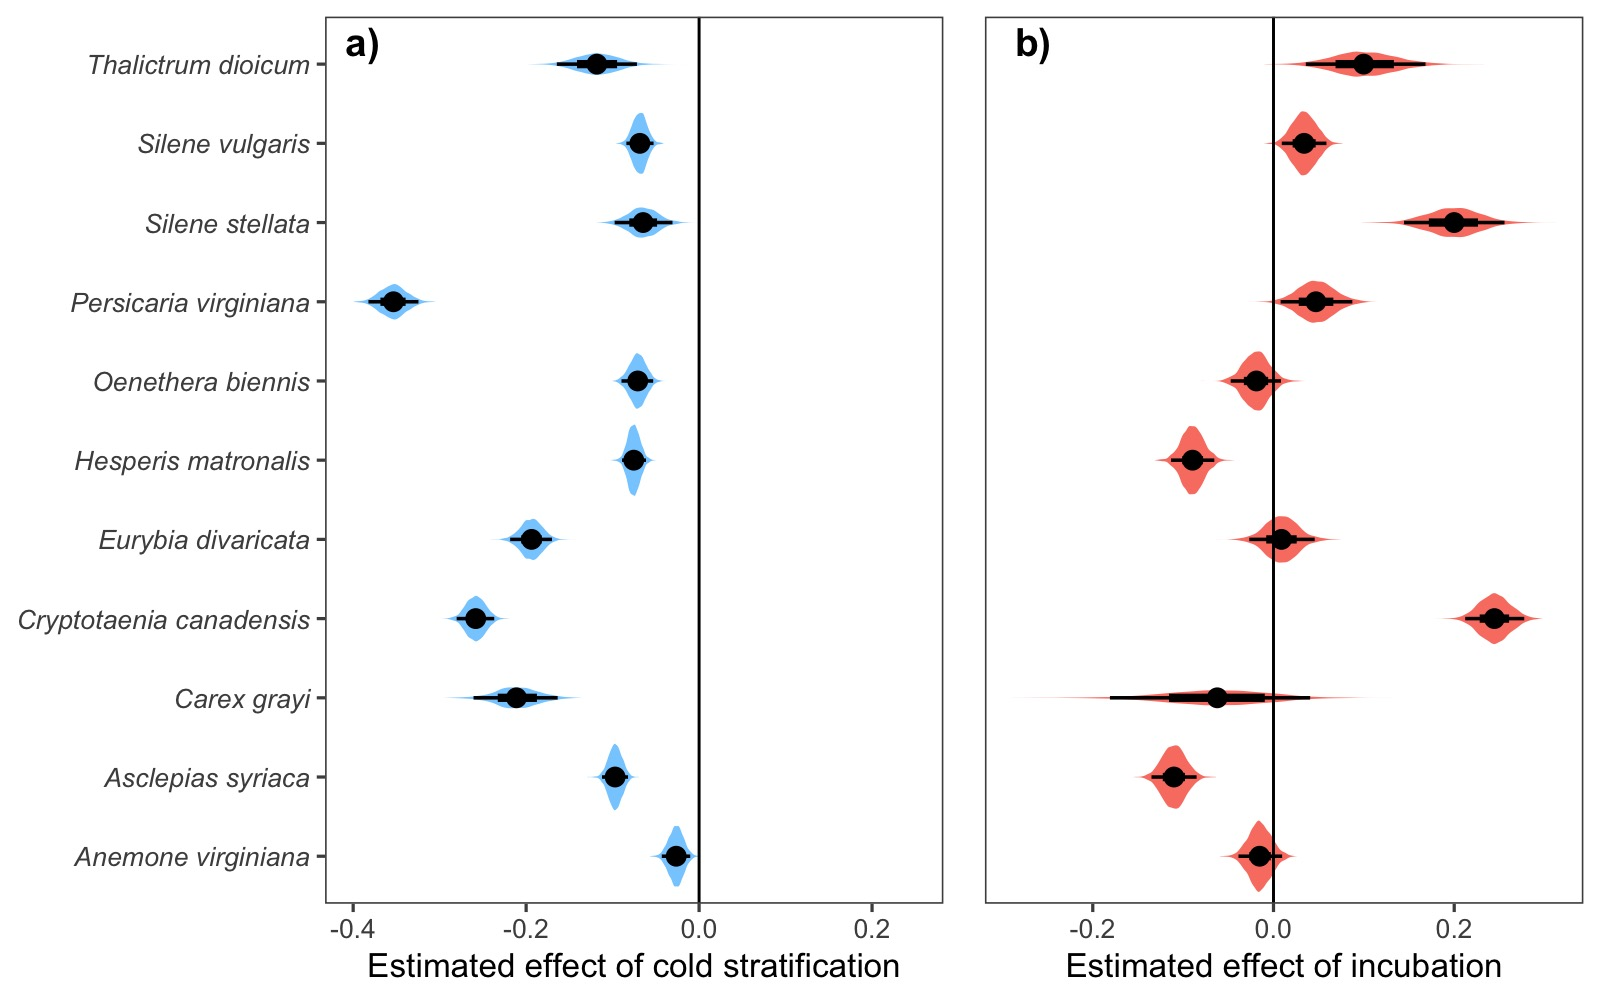
\includegraphics[width=\textwidth]{..//figure/mus_survival.jpeg}
%    \caption{Estimated effects of weeks of cold stratification (\texitbf{a)} and incubation temperature (\texitbf{b)} on the %time to 50\% germination (t50) for a suite of temperate herbaceous species. Negative estimates describe an advance in t50 and positive values a delay, estimates are on the log scale. The points indicate the mean estimated effect of each parameter, bars the  90\% uncertainty intervals, along with the full posterior distribution for each parameter as a full measure of uncertainty.} 
 %  \label{fig:musurv}
%\end{figure}


\begin{figure}[h!]
    \centering
         %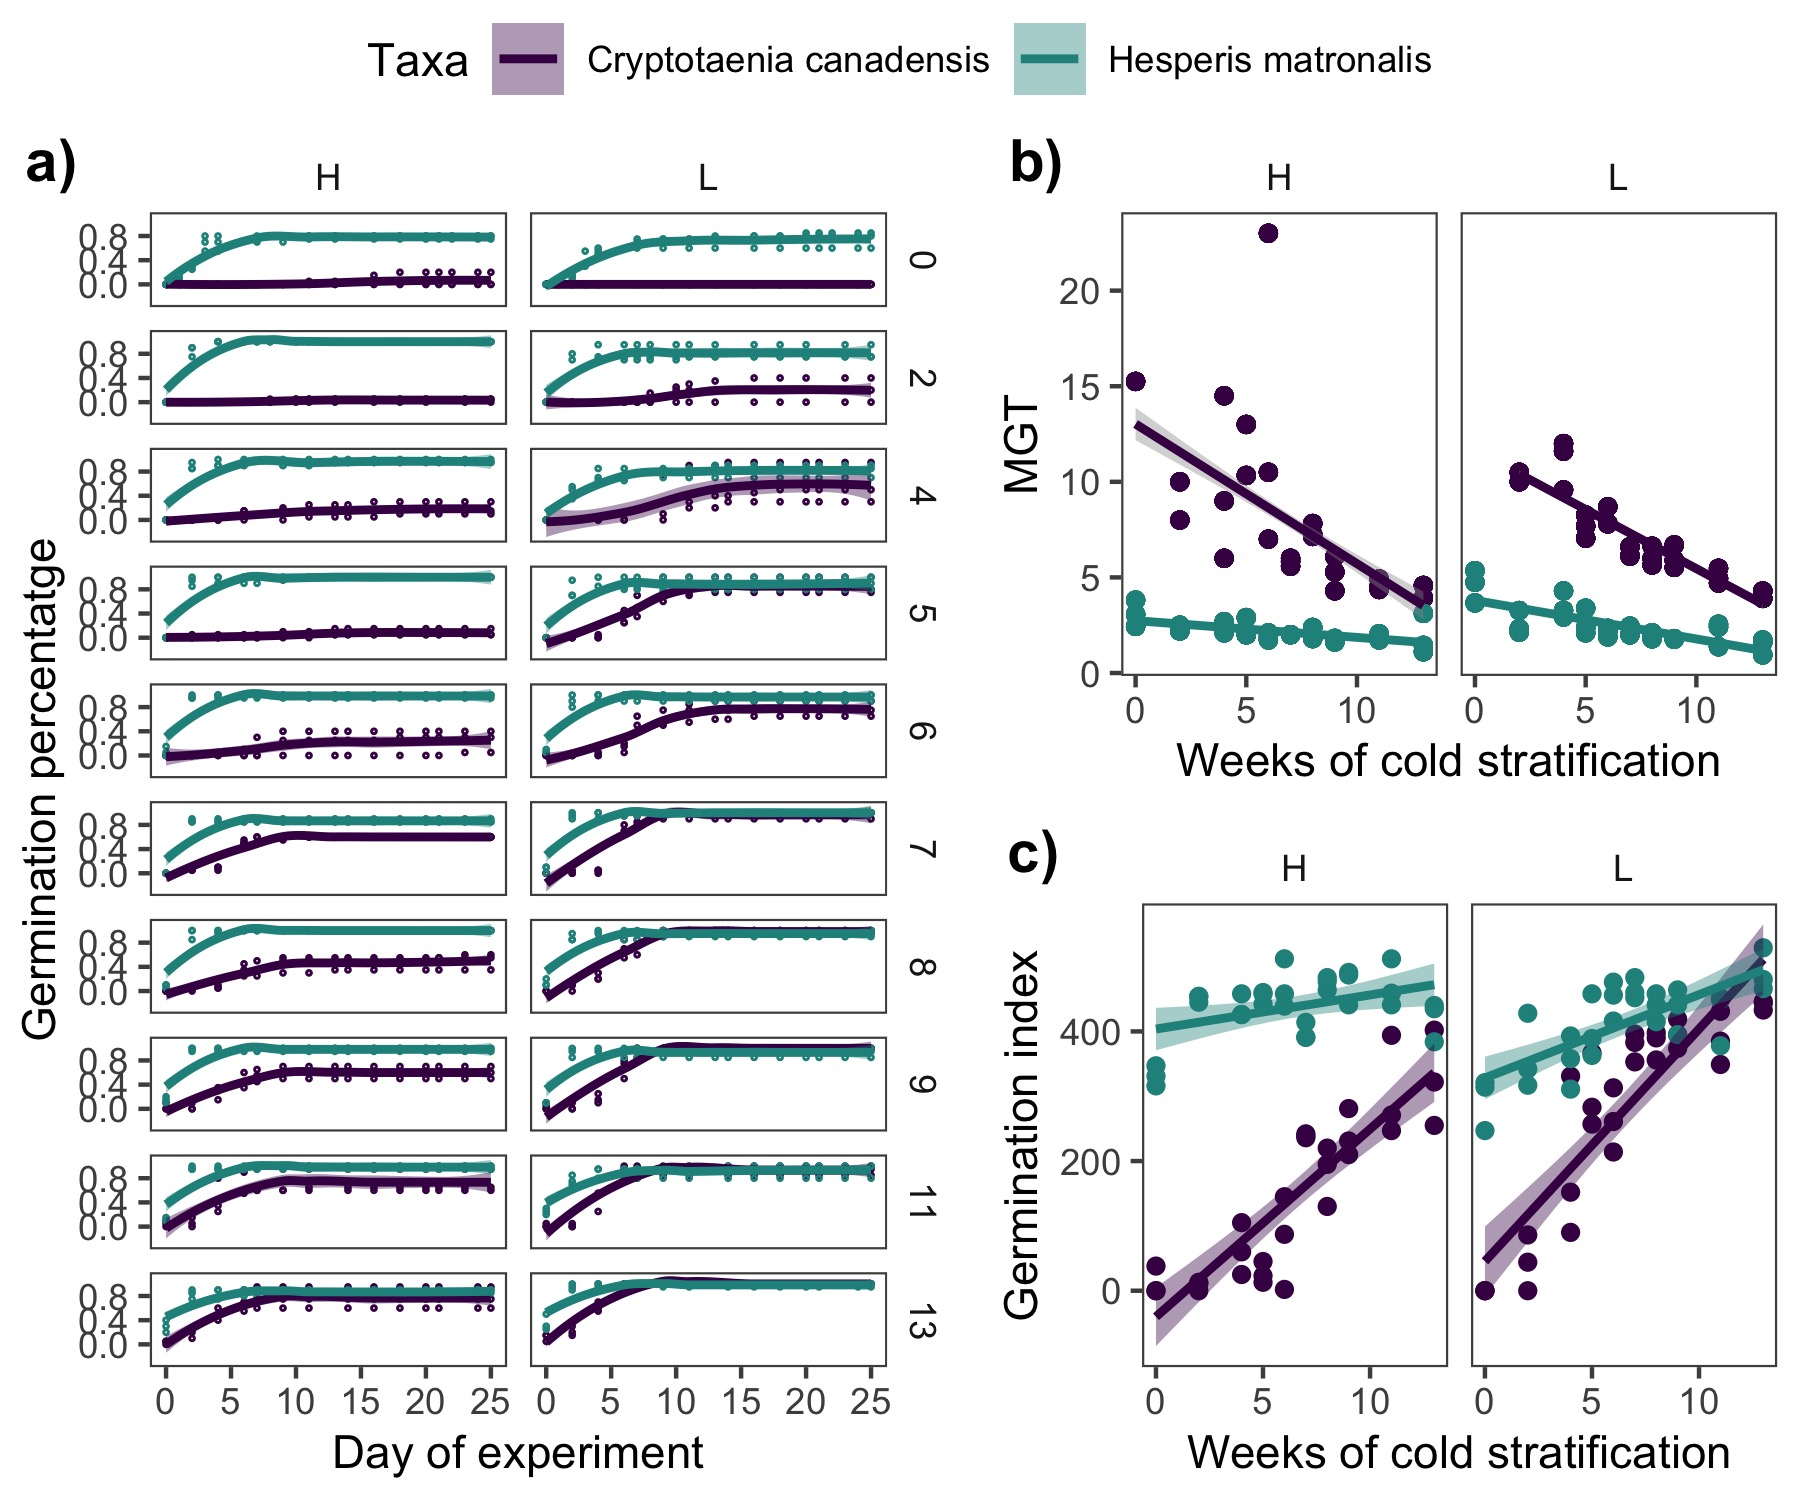
\includegraphics[width=\textwidth]{..//figure/crp_hesp1.jpeg}
          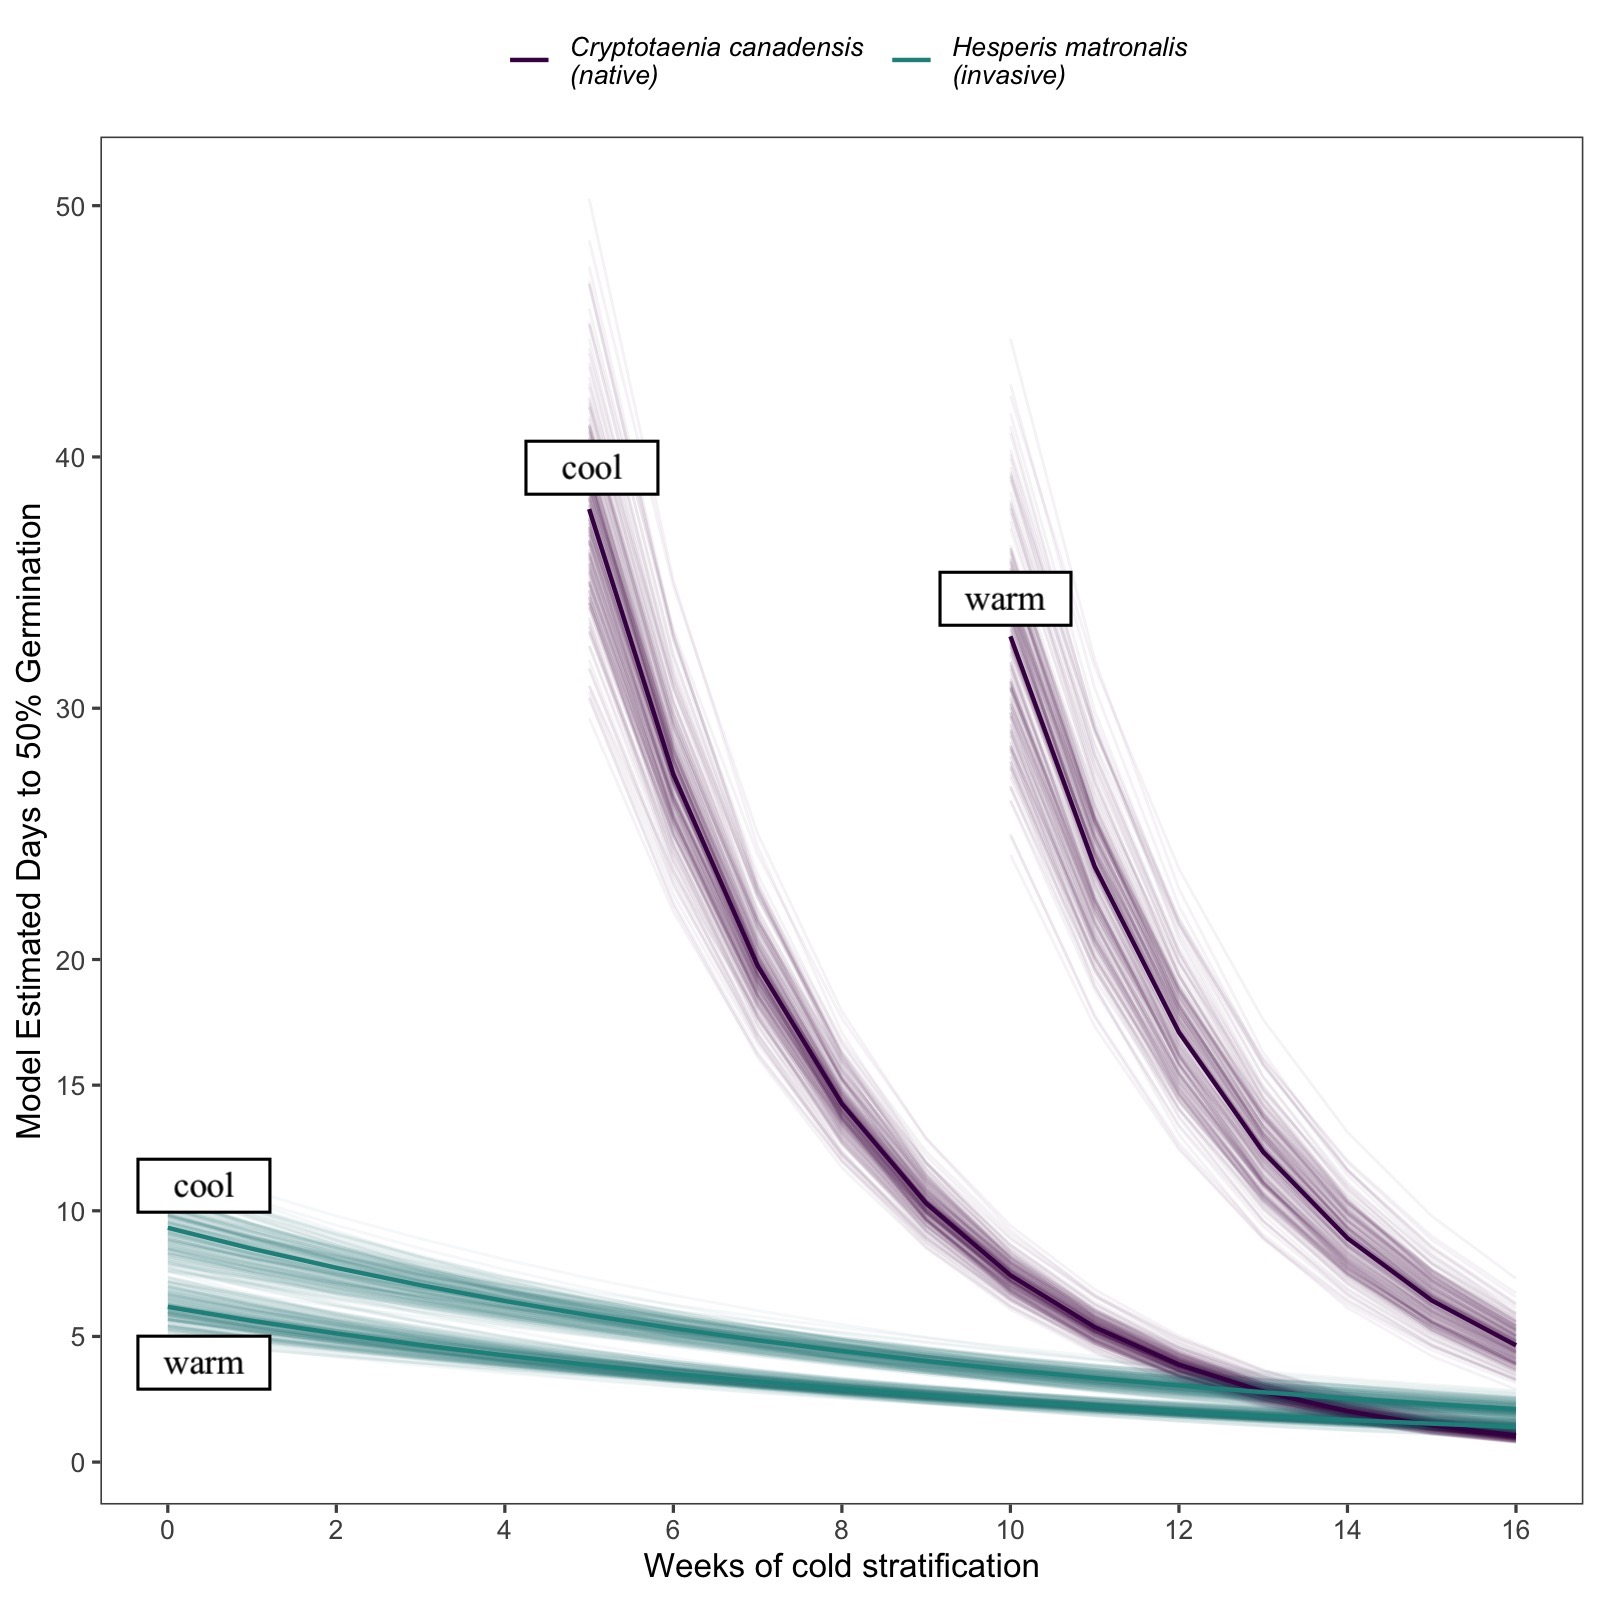
\includegraphics[width=\textwidth]{..//figure/AFTsivansive.jpeg}
%    \caption{Germination behavior of \textit{H. matronalis} and \texit{C. canadensis} indicate that the rate of \texit{C. canadensis} approaches that of \textit{H. matronalis} under cool temperatures and high levels of stratification. a) Shows germination time courses for both species at each level of incubation (H,L) and stratitification (0-13, y-axis). b) Dipicts Mean germination time for each species as a function of weeks of stratifcation and both high (H) and low (L) incubation temperature. c) Show a composite germination index for each species that account for the speed and percentage of germination for each species as a function of weeks of stratifcation and both high (H) and low (L) incubation temperature. } 
\caption{The effects of weeks of cold stratification at 4$^{\circ}$ C on the time to 50\% germination of \textit {Cryptotaenia canadensis} and \textit{Hesperis matronalis} under warm (20/10$^{\circ}$ C day/night) and cool (25/15$^{\circ}$ C day/night) incubation conditions, estimated with accelerated failure time model. We show here only stratification treatment levels which allowed both species to reach 50\% germination in less that 40 days. The solid lines depict the mean estimate, while lighter lines depict uncertainty.} %with 100 random draws from the posterior distribution.}
    \label{fig:aft}
\end{figure}


\begin{figure}[h!]
    \centering
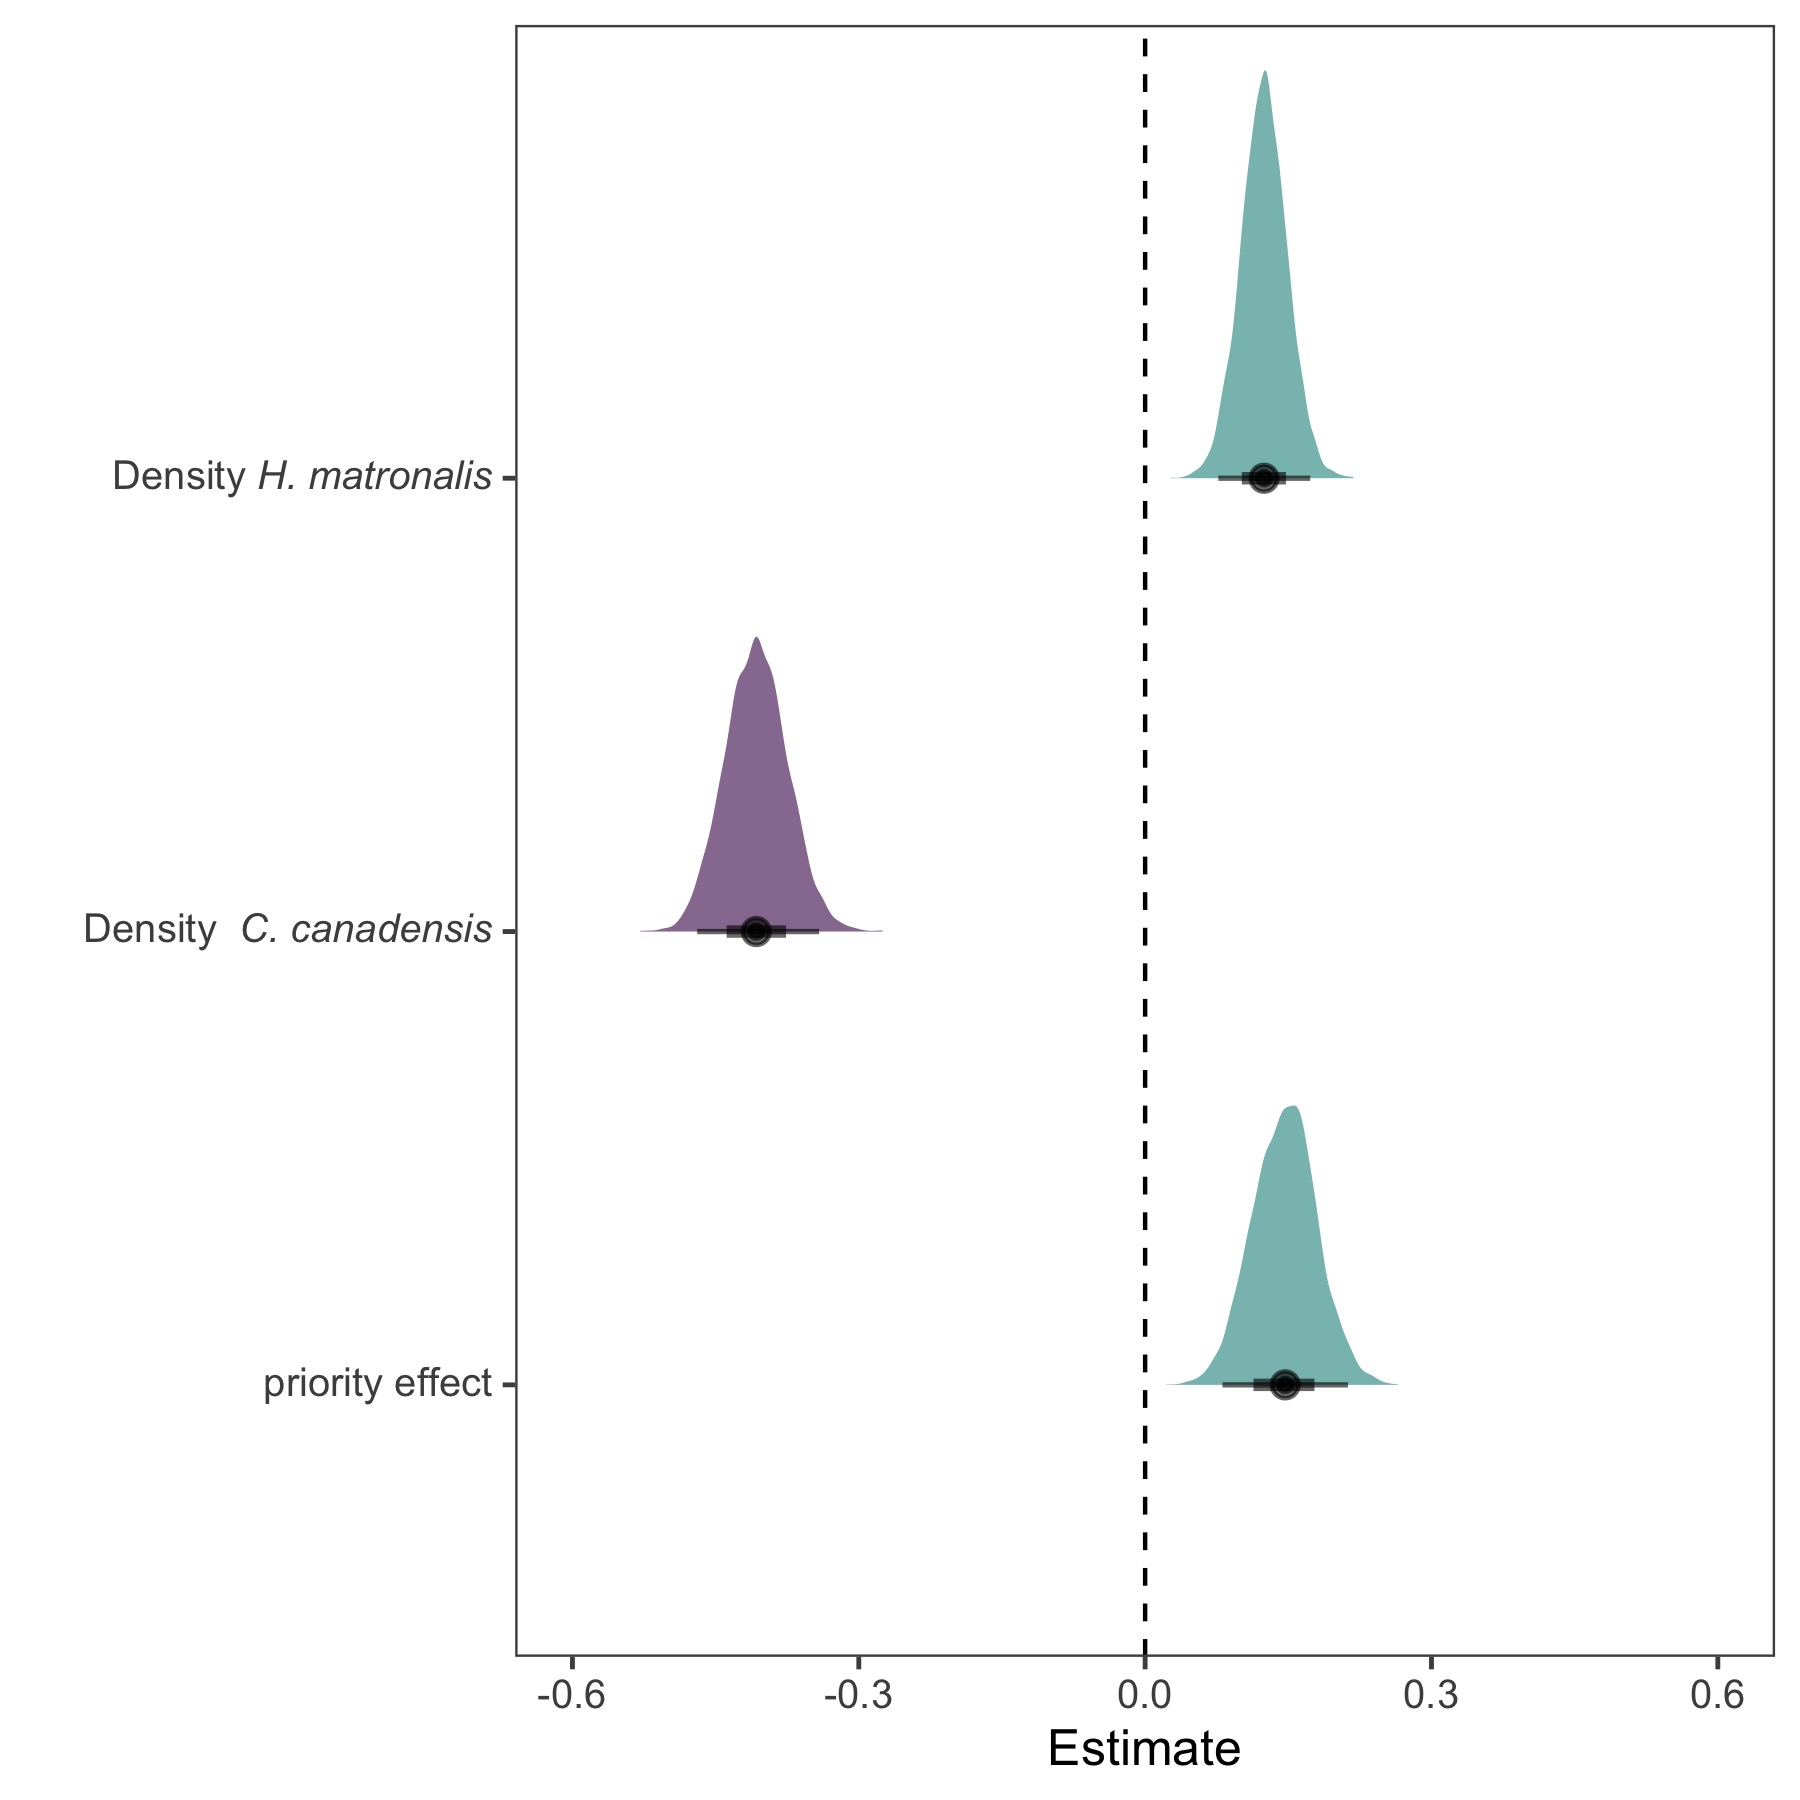
\includegraphics[width=\textwidth]{..//figure/mu_plots.jpeg}
    \caption{Estimated effects of species' abundance (intrinsic competitive ability parameters) and phenological advantage (seasonal priority effects) on the relative growth rate difference between \textit{H. matronalis} and \textit{C. canadensis}. Negative parameter estimates indicate the community biomass composition shifts to favor \textit{C. candensis} while positive estimate towards dominance by \textit{ H. matronalis}. The points indicate the mean estimated effect of each parameter and bars the 90\% uncertainty intervals. The full posterior distribution for each parameter is also depicted as an additional measure of uncertainty.} 
    \label{fig:RGRD}
\end{figure}

%\begin{figure}[h!]
 %   \centering
%\includegraphics[width=\textwidth]{..//figure/3dconnolly2.png}
%   \caption{Predicted outcome of competition under differing combinations of \textit{C. canadensis} and \textit{H. matronalis} abundance and phenological advantage of \textit{H. matronalis}. Purple dots indicate conditions that favor  \textit{C. canadensis} in community biomass composition while green dot conditions favor \textit{H. matronalis}. Estimates are based on multiple regression models estimating the effect of each variable on the relative growth rate difference among species.} 
 %  \label{fig:3D}
%\end{figure}

\begin{figure}[h!]
    \centering
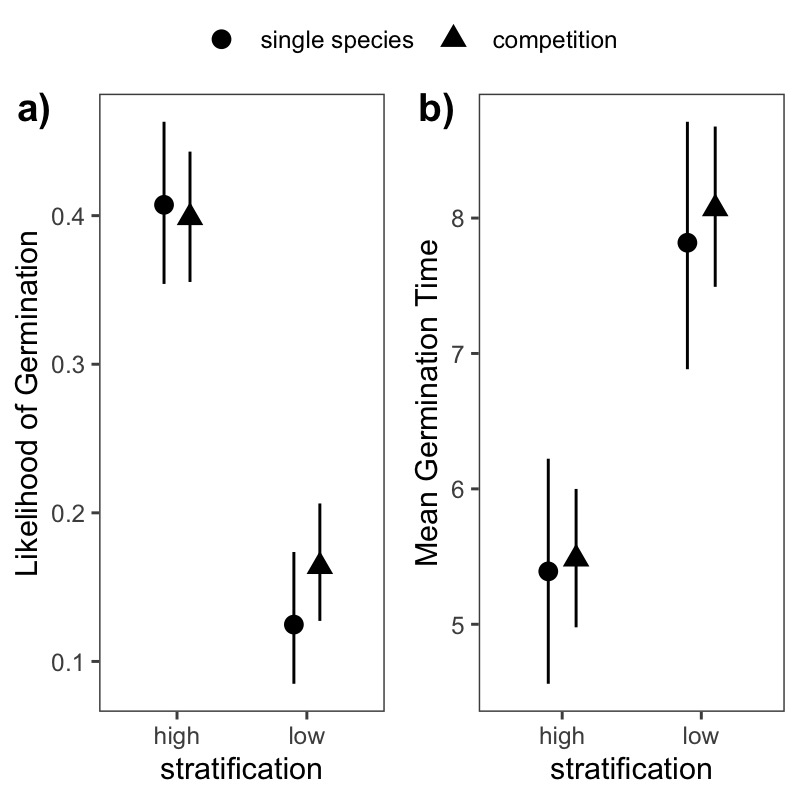
\includegraphics[width=.7\textwidth]{..//figure/nichemodfication.jpeg}
   \caption{Estimated effects of single and mixed species competition on the germination dynamics of \textit{Cryptotania canadensis} under 6 (low) and 10 weeks (high) of cold stratification at 4$^{\circ}$C. Panel \textbf{a)} depicts differences germination likelihood and \textbf{b)} shows the estimated mean germination time in single species vs. competition pot. Points represent the mean estimates under each planting type and bars represent 90\% uncertainty intervals. } 
   \label{fig:nichemod}
\end{figure}

%\begin{figure}[h!]
 %   \centering
%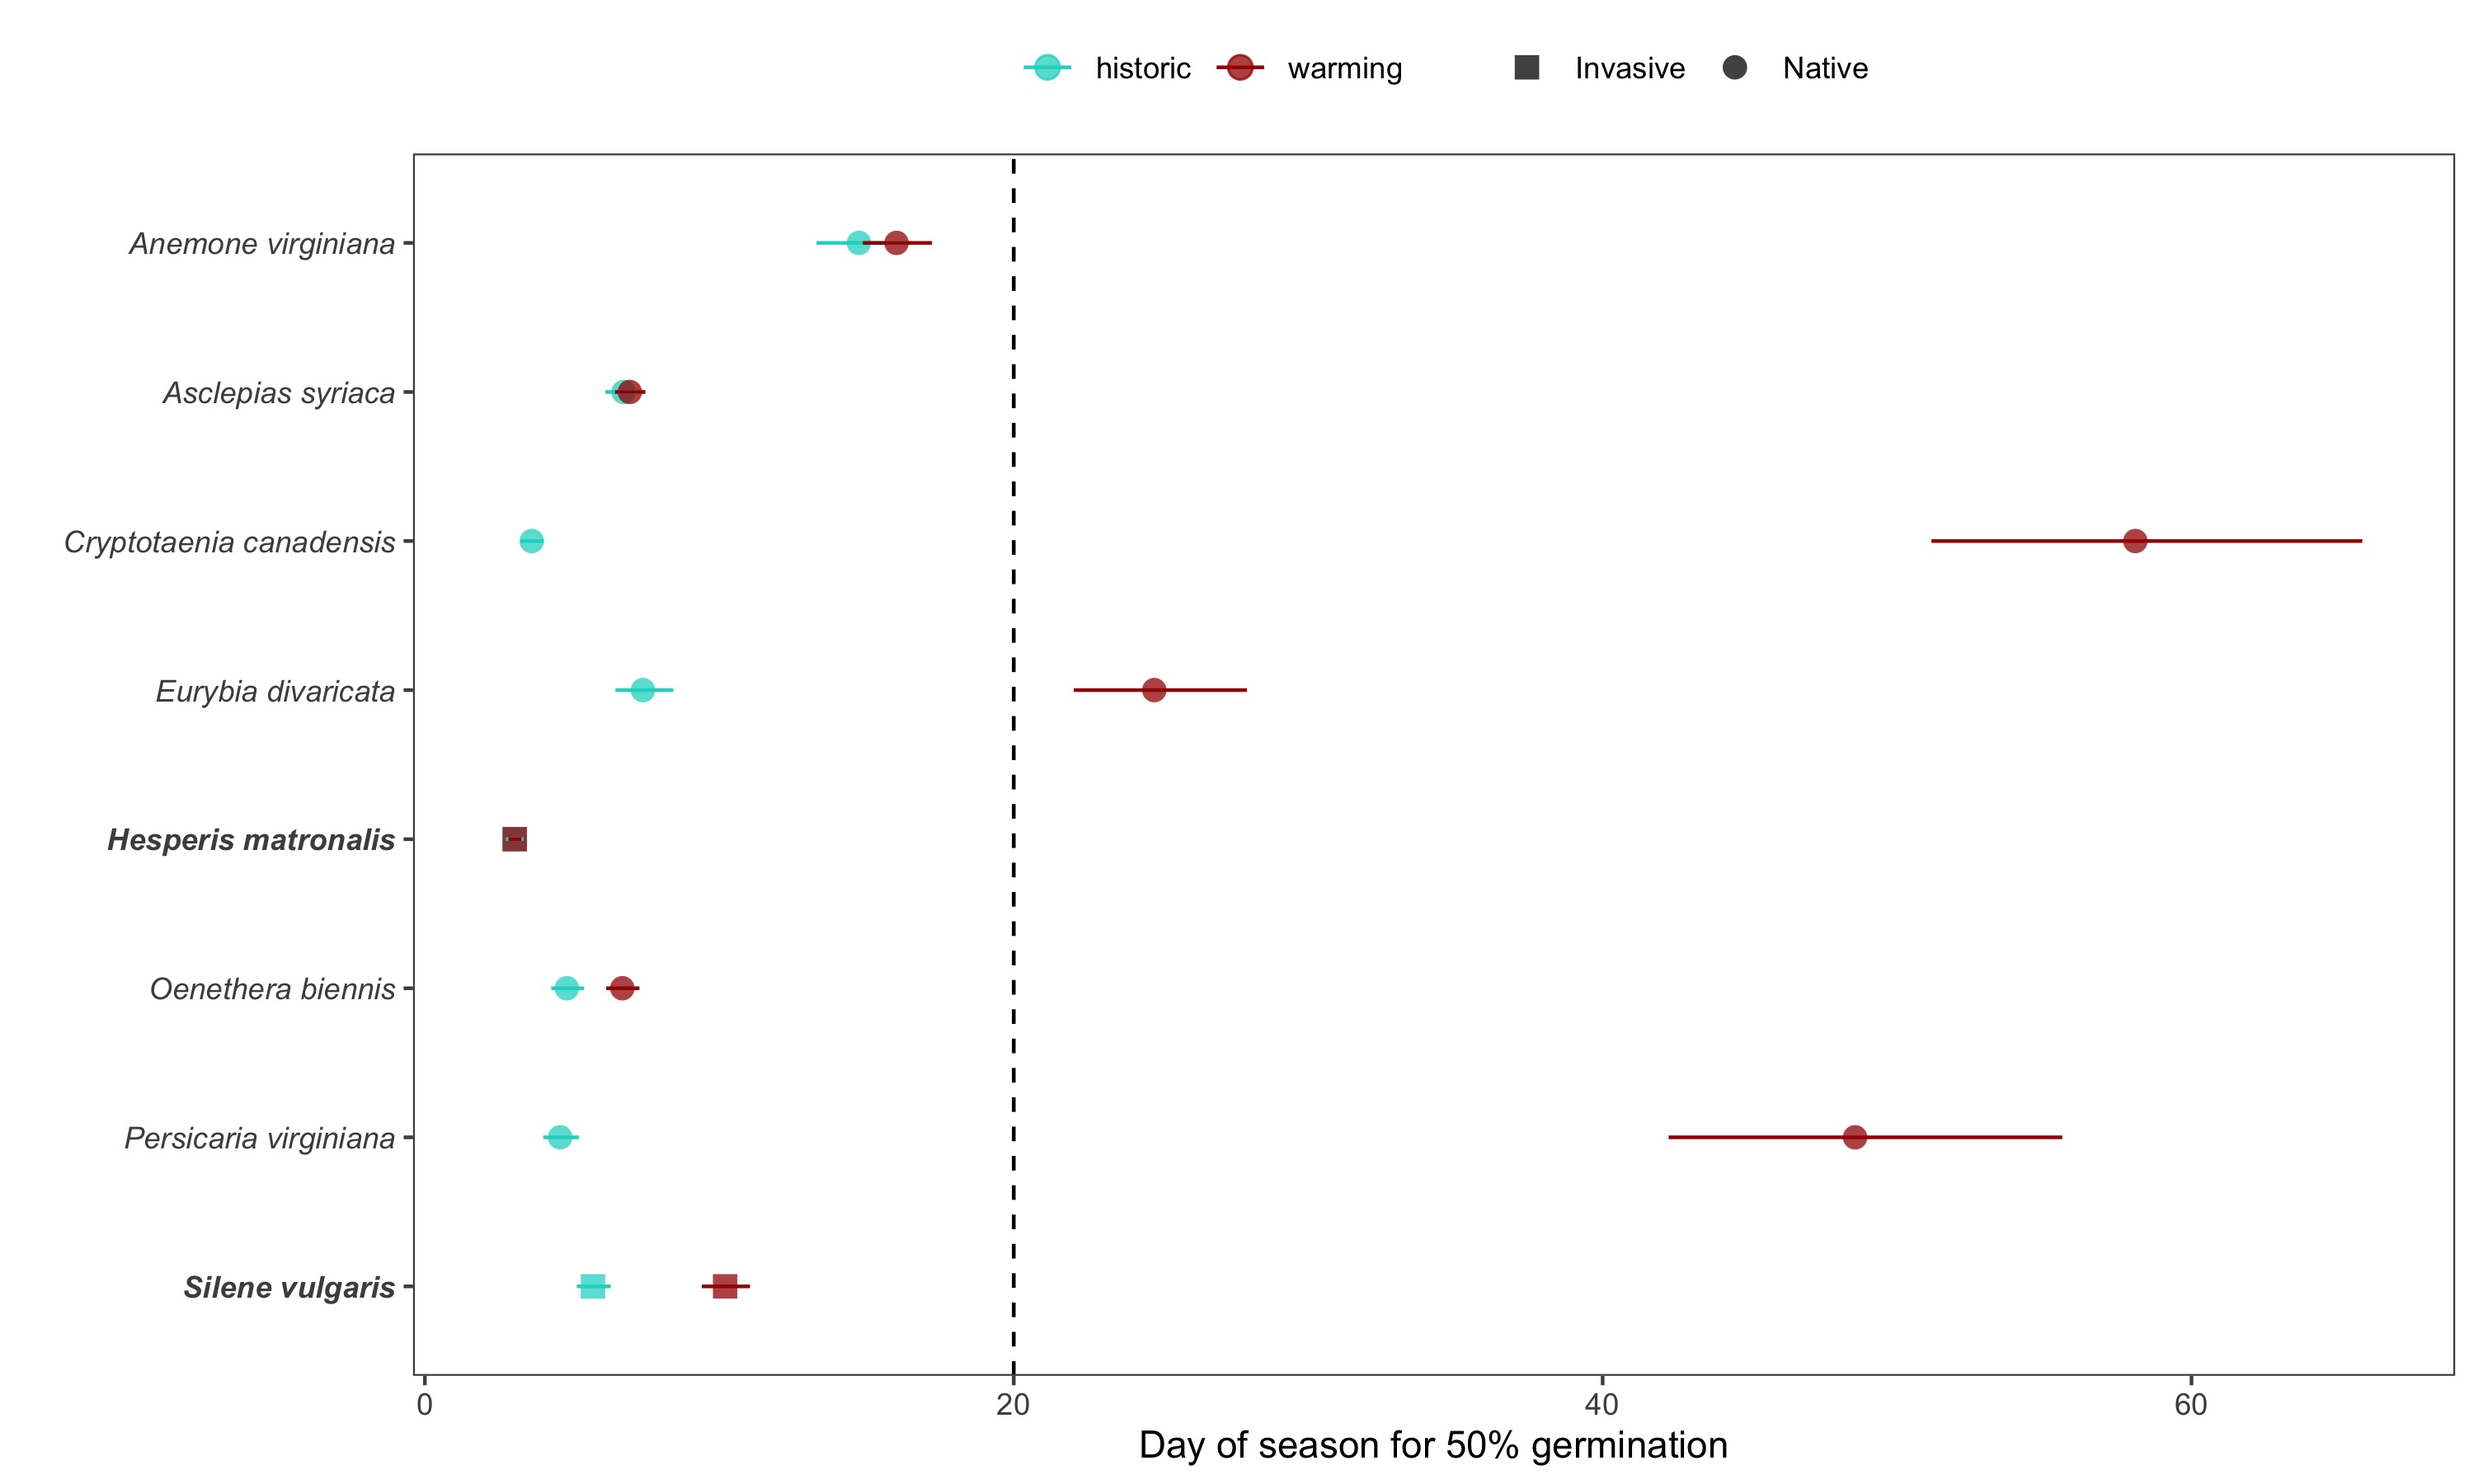
\includegraphics[width=\textwidth]{..//figure/commchange.jpeg}
%   \caption{Predicted germination phenology of a suite of temperate herbs under historic (12 weeks cold stratification at 4$^{\circ}$C and  20/10$^{\circ}$ incubation)  and climate warming scenarios (6 weeks cold stratification at 4$^{\circ}$C and  25/15$^{\circ}$ incubation).  Warming reduces the ratio of native to invasive species that germinate within 20 days of the growing period, and increases the phenological advantage of the invasive species in this study. Points represent mean estimates of time to 50\% germination and bars represent 90\% uncertainty intervals. } 
%   \label{fig:comm}
%\end{figure}


\end{document}

